%!TEX root = main_thesis.tex
%---------------------------------------------------------------------------------
\chapter{An Architecture for Multi-Standard Cognitive Radios}
\label{chap:MSCR}
%---------------------------------------------------------------------------------
\definecolor{F1}{HTML}{a1dab4}
\definecolor{F2}{HTML}{225ea8}
\definecolor{F3}{HTML}{41b6c4}
%---------------------------------------------------------------------------------
\section{Introduction}
%---------------------------------------------------------------------------------
Cognitive radios that support multiple bands, multiple standards and adapt operation according to environmental conditions are becoming more attractive as the demand for higher bandwidth and more efficient spectrum use increases.
Traditional implementations in custom ASICs cannot support such flexibility, with standards changing at a faster pace, while software implementations of baseband communications fail to achieve the performance required.
Hence, FPGAs offer an ideal platform bringing together flexibility, performance, and efficiency.
In this chapter, we show how we can incorporate our contributions in previous chapters into a flexible architecture for multi-standard cognitive radios (MSCR).
We show that combining partial reconfiguration (PR) with parameterised  modules offers flexibility while minimising reconfiguration time.
\todo[inline]{When the system adapts to a new condition (i.e., switching the operating standard), a reconfiguration operation is performed which may pause or suspend data processing for the duration of the reconfiguration. Received packets of data may therefore be lost. 
The reconfiguration is required to operate fast enough that the input data buffered during reconfiguration does not overflow the buffer, leading to entire packets of data being dropped. Even though there are higher-level protocols available to manage the retransmission of lost or dropped packet of data, performing these mechanisms is wasteful and may significantly increase the cost in terms of computation and power consumption.'}

The work presented in this chapter has also been discussed in:
\begin{itemize}
\item T. H. Pham, S. A. Fahmy, and I. V. McLoughlin, ``Efficient Multi-Standard Cognitive Radios on FPGAs,'' PhD Forum Poster in \textit{Proceedings of the International Conference on Field Programmable Logic and Applications (FPL), Munich, Germany, September 2014}~\cite{Pham2014a}.
\item T. H. Pham, S. A. Fahmy, and I. V. McLoughlin, ``Efficient OFDM-based baseband processing for Multi-Standard Cognitive Radios on FPGAs,'' in preparation for submission to \emph{ACM Transactions on Embedded Computing Systems}.
\end{itemize}

%---------------------------------------------------------------------------------
\section{Related Work}
%---------------------------------------------------------------------------------
Most practical CRs are built using powerful general purpose processors to achieve flexibility through software, but they can fail to offer the computational throughput required for advanced modulation and coding techniques and they often have high power consumption.
GNU Radio~\cite{gnuradio} has been a widely used platform in academia.
It is a software application that runs on a computer or an embedded ARM processor platform, e.g. on the Ettus USRP E100.
Computational limitations mean that while it has been successful for investigating CR ideas, it is not feasible for implementing advanced embedded radios using complex algorithms.
Other software based frameworks like Iris~\cite{Sutton2010}, have some limited support for FPGAs but suffer from poor bandwidth between software and hardware.
Moreover, the compilation time and reconfiguration time of software defined radio systems can be long making them unsuitable for adapting to fast changing conditions.

In an application area with fast moving standards and requiring support for multiple standards, custom ASIC implementation is unlikely to be agile or cost effective enough to cope with fast-changing standards and operating requirements.
In order to address this, Delorme et al.~\cite{Delorme2008} presented a heterogeneous reconfigurable hardware platform for Cognitive Radio.
It can adapt its hardware structure to support standards like GSM, UMTS, and wireless LAN.
Most processing components run as embedded software on the nodes in a network-on-chip processor, while the channel coder and the mapping of the RX chain are implemented inside an FPGA.
Partial reconfiguration (PR) is used to switch the channel coder from one context to an another depending on SNR.
A processor manages data movement between the different processors, the ASIC, and the FPGA. The need for a large data buffer and inefficient data transfer mechanisms results in increased power consumption and reduced throughput.

Other platforms do not propose specific methods for managing a radio's dynamic behaviour.
KUAR~\cite{Minden2007} is a mature radio platform built around a fully-featured Pentium PC with a Xilinx Virtex II FPGA.
The baseband processing is accelerated on FPGA and limited to NC-OFDM waveforms based on the IEEE 802.16 standard.
Projects at Virginia Tech~\cite{athanaswires} have shown dynamically assembled radio structures on FPGAs, where the target radio system is defined at a high-level with datapaths connecting relatively large functional modules.
The modules are wrapped, and each of them consists of a PR module with complied partial bit-streams stored in dynamic library.
Their online assembly method eliminates the need for run time compilation, thus affording flexibility.
A flexible radio controller can insert and remove compiled modules to adapt to current conditions.
However, by using low-level reconfiguration circumventing the official PR flow, it is unclear how this approach can be mapped to newer architectures as they appear.

%---------------------------------------------------------------------------------
\section{Proposed OFDM Baseband for MSCR}
%---------------------------------------------------------------------------------
\begin{figure}
%\centering
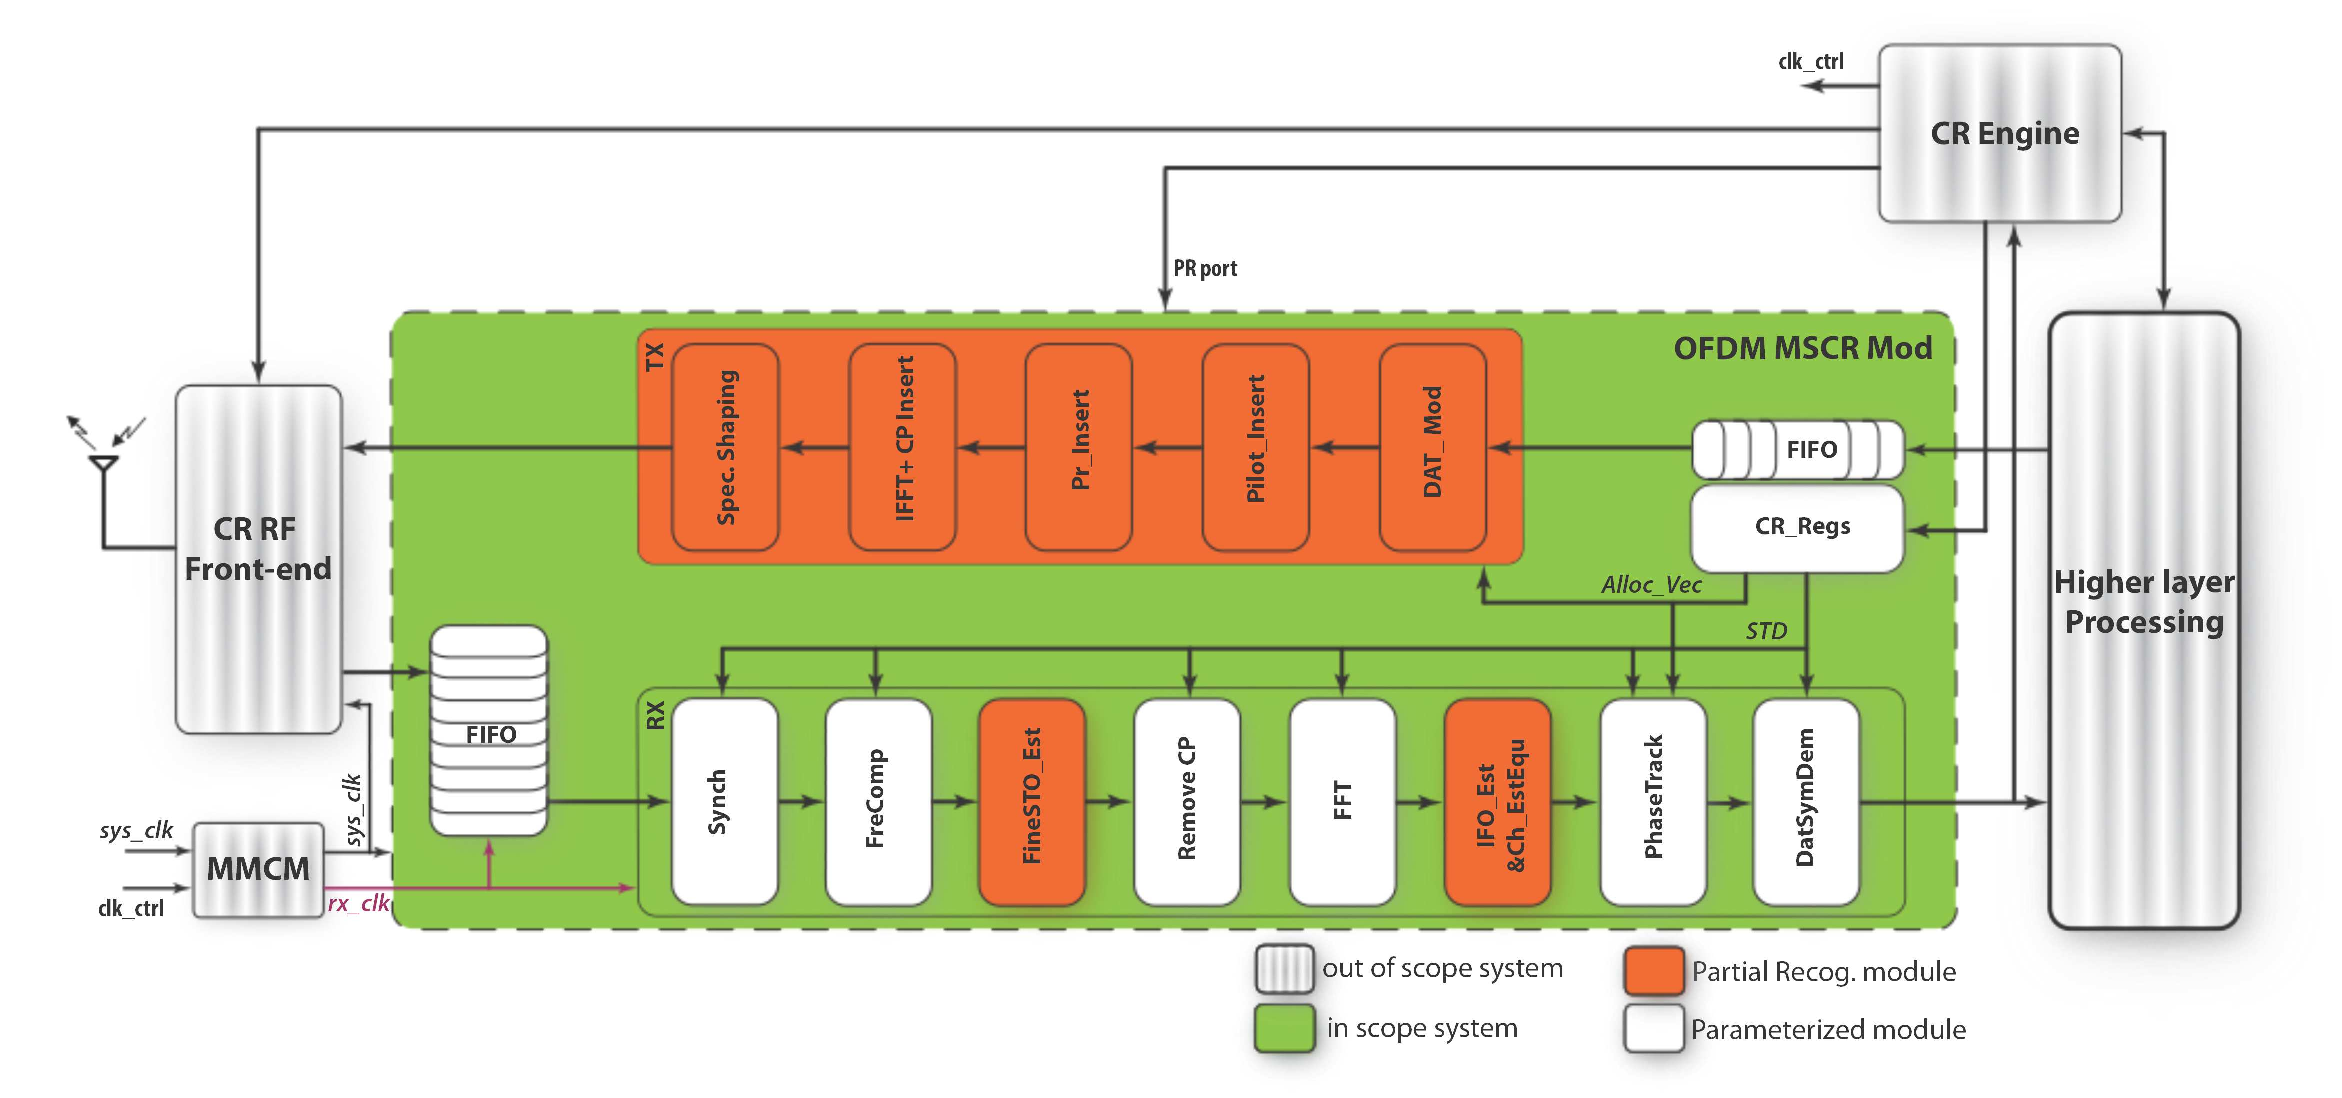
\includegraphics[width=1.05\columnwidth]{Figures/MSCRFig.eps}
\caption{The structure of a generic MSCR system}
\label{fig:struc}
\end{figure}

Fig.~\ref{fig:struc} illustrates the proposed structure of baseband modulation for our OFDM-based MSCR.
A mix of partially reconfigurable and parameterised modules make up the baseband implementation.
FIFOs are included to help overcome the reconfiguration latency when PR modules are reconfigured.
While a sink module is reconfiguring, these FIFOs store samples from the source until the module is ready to process data.
Since these modules are now just a small part of the system, buffering is significantly reduced over a more general implementation.

\subsection{System Description}

We developed a prototype MSCR baseband that supports transmitting and receiving non-contiguous OFDM (NC-OFDM) signals.
This system can perform with different OFDM symbol lengths and frame formats specified differently according to multiple standards such as IEEE~802.11~\cite{IEEE80211}, IEEE~802.16~\cite{IEEE80216}, and IEEE~802.22~\cite{IEEE80222}.
The main specifications of these standards are summarised in Table~\ref{Tab:spec}.

\begin{table}[h]
\centering
\caption{System specifications of three supported OFDM-based standards.}{
\renewcommand{\arraystretch}{1.3}
\begin{tabular}{@{}llll@{}}
\toprule
Specifications 			& IEEE~802.11 				& IEEE~802.16				& IEEE~802.22 		\\ \midrule
Frequency band			& 2.4--2.5~GHz				& 5--6~GHz					& 54--862~MHz		\\
Channel Width			& 10~MHz					& 10~MHz					& 8~MHz			\\
Sampling Frequency		& 10~MHz					& 11.52~MHz				& 9.136~Mhz		\\
FFT size ($N$)		& 64						& 256						& 2048			\\
CP Length				& 16						& 32						& 512				\\
Number of data carriers		& 48						& 192						& 1440			\\
Number of pilots			& 4						& 8						& 240				\\
\end{tabular}
\label{Tab:spec}
}
\end{table}

The CR implementation is divided into a control plane and data plane.
The data plane performs data processing on the sample data stream.
It tranceives data streams to/from the RF front end through two AXI (Advanced eXtensible Interface) stream interfaces.
For transmission, data is sent from higher layers and modulated by the data plane.
Modulated sample streams are then transferred to the RF front end to convert to analogue signals and subsequently up-converted before transmission on the RF channel.
For the receiver side, the received signals are down-converted to the baseband followed by analogue to digital conversion to form a sample stream.
The sample stream is demodulated and processed in the data plane before being transferred to a higher layer.

To support multiple standards, the data plane must provide the flexibility of switching baseband modules to the parameters specified by different standards.
AXI Stream interfaces are used for inter-module communication in the data plane as well as for communication with software.
With partial reconfiguration, modules that that swap into the same region must share the same interfaces, so this is a suitable abstraction.
The AXI Stream protocol also reduces the requirement for buffering, hence optimising resource usage and total power consumption~\cite{Liu2009}.
Each module has one slave interface to receive data from the previous module and one master interface to send processed data to the subsequent module.

The control plane is a cognitive radio (CR) engine that is required to perform adaptive based on the requirements of the application, ultimately deciding which base standard to use, and which sub-carriers to enable.
A bus register interface between the control and data planes allows them to communicate.
The CR engine also includes the PR controller that is responsible for loading bitstreams stored in DRAM into the corresponding PR regions through the ICAP (Internal Configuration Access Port) interface~\cite{Vipin2012} when necessary.

The control plane can be implemented in a number of ways.
It can be standalone software running on a processor core. It can also be hardware in a separate part of the FPGA.
Alternatively, for maximum flexibility and programming support, it can run on top of an operating system on the processor.
By ensuring that symbol data is processed and moved through the data plane independently of the processor in the control plane, we are able to achieve high throughput.
Normally, the data plane processes data streams based on a specified standard.
An allocation vector determines which sub-carriers to enable, allowing the radio to respond to varying channel occupancy conditions.
When the frequency band of the current operating mode is mostly occupied by PUs and IUs, the CR engine instructs the baseband to switch to another standard or frequency band that is currently (or will soon be) free for transmission.
The PR controller inside the CR engine is required to download the bitstreams of PR modules according to the new standard.
In the meantime, the CR engine configures the system by writing relevant parameters to registers in $CR\_Regs$ such as allocation vectors (Alloc\_vec), symbol modulation type (MOD), and standard (STD).

The scope of this chapter focuses on the managing the baseband adaptation in a way that avoids long configuration time.
We do not explore the cognitive functions, nor discuss sensing, which can be implemented in a variety of ways.
The system takes advantage of combining PR with parameterised modules to offer flexibility while minimising reconfiguration time.
The CR system is designed to be capable of operating in burst mode in which it transmits packets as soon as data is available~\cite{Ai2006}.
If a data packet is ready to be sent but reconfiguration is in progress, it is buffered in a FIFO.
It is then flushed out of FIFO for transmission after reconfiguration is completed.
Since the resource requirements for the transmitter are significantly less than the receiver, reconfiguration time is also shorter.
We discuss the resource utilisation and reconfiguration time of the transmitter in Section~\ref{sec:PerAna}.
Short reconfiguration time means there is no critical disruption of the processing chain and loss of transmitted packets.
Hence, for the transmitter, we use a single PR region with the whole transmission chain for simplicity and flexibility.

The receiver subsystem, by contrast, is required to continuously receive and process data frames.
Furthermore, the hardware usage of the receiver subsystem is much larger than the transmitter, resulting in longer reconfiguration time.
One way to avoid losing data frames, is to use a large FIFO to store received samples from the RF front end during reconfiguration, but this can be problematic as this results in significant resource usage.
Our aim here is to reduce reconfiguration time in the receive chain to mitigate the need for such large FIFOs.

We propose making some modules parameterised, while others are reconfigured using PR.
We explore how to optimise this mix in Section~\ref{sec:7module}.
Now smaller FIFOs can be used and reconfiguration can be applied at a finer granularity to minimise the impact of reconfiguration on buffer storage requirements.
After reconfiguration is complete, it is necessary to flush the FIFOs and ``catch up'' with the received samples.
This can be done by increasing the processing clock rate until the FIFOs are no longer full.
%A Mixed-Mode Clock Manager (MMCM) is used for this purpose, modifying the processing clock (rec\_clk) to a higher frequency.
\todo[inline]{Increasing operating speed is done basically by controlling the MMCM module to adjust the speed of the input clock of the receiving modules, rx\_clk. Because these modules implemented on FPGA fabric are able to work with a clock that is higher than 2X the operating clock, designing these modules to support twice the normal operating clock does not consume more resources compared to the case of the normal clock speed.}
It is then reduced back to the sampling rate (sys\_clk) to reduce power consumption.
The MMCM module is also required to change the processing rate of data plane according to the different sampling rates specified in different standards, shown in Table~\ref{Tab:spec}.

\subsection{Module Description}\label{sec:7module}

In this section, we detail the design of each functional module shown in Fig.~\ref{fig:struc}, showing how to build a multi-standard implementation.
There is a tradeoff between the simplicity, flexibility, but long reconfiguration latency of a PR module and the increased hardware overhead, complexity, but faster configuration of a parameterised module.
The comparison between the hardware usage of parameterised modules for multiple standards and that of individual specified standard modules is evaluated.
In cases where the hardware overhead for parameterisation is a threshold of the maximum area of a stand-alone module, it is judged as better parameterised.
For those modules that require significant changes (i.e. the parameterised overhead is greater than this threshold) or are required to support unspecified parameters for future standards (such as the preamble), PR can be used on a per-module basis.
Separate bitstreams for each implementation are generated to be mapped to a PR region.
Hence, when switching the entire baseband from one standard to another, only part of the FPGA needs to be reconfigured.

\subsubsection{FIFO Buffer (FIFO)}
There are two FIFOs at the transmitter side and the receiver side to buffer data sent from the higher layer and the RF front end, respectively.
The FIFO buffers are implemented using Xilinx FIFO IP cores with 2 port AXI stream interface configuration.
In the normal operation of data stream, one data word is written to the buffer by the higher layer/the RF front end, while another one is read out from the buffer by the transmitter side/receiver side in each system clock cycle.
Therefore, the FIFOs normally operate in an almost empty state.
When reconfiguration is required to switch the baseband, the transmitter processing and receiver processing are suspended.
The FIFO buffers store incoming data to avoid losing frames.
Because the system performs in burst mode, the transmitter streams are not continuous, therefore, the transmitter FIFO can flush stored data during  gaps between bursts.
The data buffer is not a critical issue for the transmitter side.

The receiver must, however, process continuously to detect incoming frames, and so, there is no spare time to flush data that has been buffered in the FIFOs during reconfiguration.
Therefore, the receiver FIFO is configured with independent clocks as shown in Fig.~\ref{fig:FIFO}.
In order to flush stored data in the received FIFO after reconfiguration, the MMCM increases the receiver processing rate (rx\_clk) to be higher than the sampling rate of the RF front end to help empty the FIFO faster.
Once the receiver FIFO is almost empty the processing rate is returned to the sampling rate to minimise power consumption.
Since the FIFO IP cores support independent write and read clocks, this functionality is seamless to the stream processing.
\begin{figure}
\centering
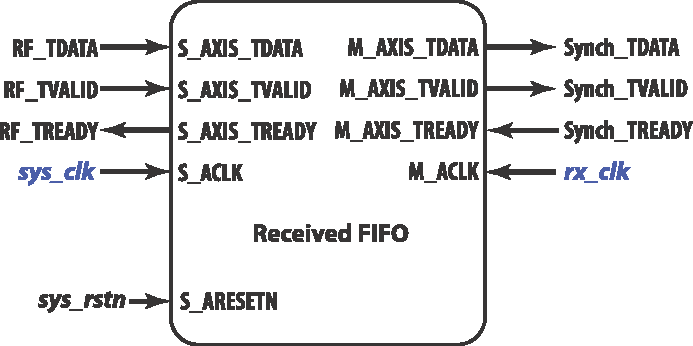
\includegraphics [width=0.5\columnwidth]{Figures/MSCR_RX_FIFO.pdf}
\caption{The receiver FIFO module.}
\label{fig:FIFO}
\end{figure}

\subsubsection{Synchronisation (Synch)}
Our CR system communicates in burst mode.
Hence, it must detect the presence of a frame and estimate the frequency offset required, based upon the preamble of the received frame.
The \emph{Synch} module performs estimation as discussed in Chapter~\ref{chap:Synchronisation}.
Fig.~\ref{fig:Sync} shows a block diagram of its implementation.

The timing metrics are calculated by using auto-correlation on received samples.
\emph{Coarse Time} detects the new frame and roughly estimates the start of a frame using blind estimation that provides generality for application to multiple standards.
By parameterising the length of $L$, the synchronisation module can effectively perform for three current supported standards as well as being extensible for future standards.

This module is implemented as a parameterised version with parameter $L$ whose values are defined together with the length of FFT ($N$), shown in Table~\ref{Tab:L}.
Combinations of $L$, and $N$ allow it to support multiple standards.
The parameterised values consist not only of the required combinations for 802.11, 802.16, and 802.22, but also support other combinations for future standards.
\begin{table}[h]
\centering
\caption{Parameterised values according to supported standards}{
\begin{tabular}{|l||*{6}{c|}}\hline
\theadset\theadfont\backslashbox[3em]{N}{L}
&\makebox[2.3em]{\thead{16}}&\makebox[2.3em]{\thead{32}}&\makebox[2.3em]{\thead{64}} &\makebox[2.3em]{128}&\makebox[2.3em]{\thead{256}}&\makebox[2.3em]{\thead{512}}\\\hline\hline
64 		& 802.11 & & & & & \\\hline
128 	& & & & & & \\\hline
256 	& & & 802.16 & & & \\\hline
512 	& & & & & & \\\hline
1024 	& & & & & & \\\hline
2048 	& & & & & & 802.22\\\hline
\end{tabular}
\label{Tab:L}
}
\end{table}

\begin{figure}
\centering
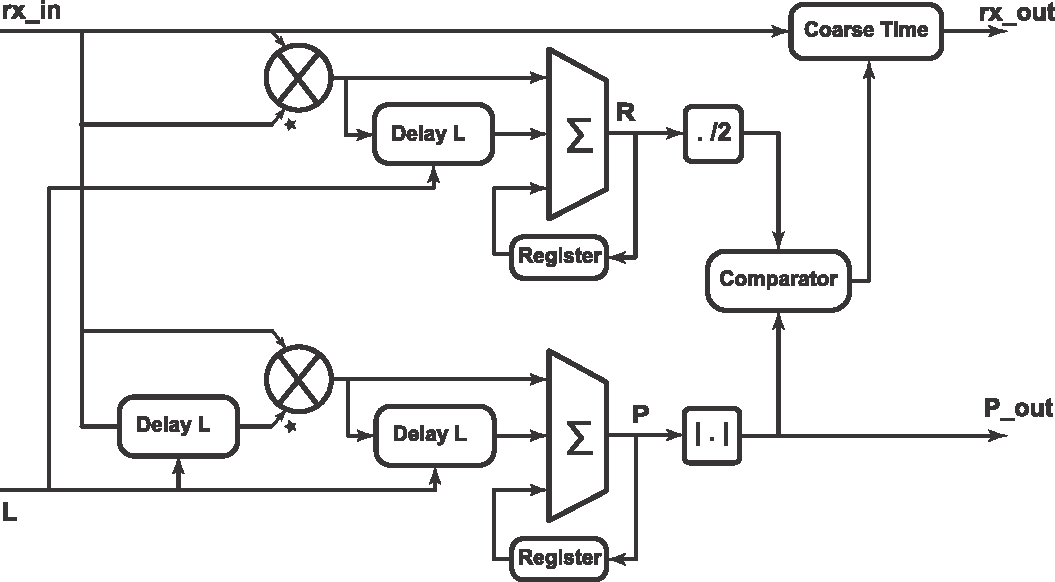
\includegraphics [width=0.7\columnwidth]{Figures/MSCR_RX_Sync.pdf}
\caption{Block diagram of Synchronisation module.}
\label{fig:Sync}
\end{figure}

\subsubsection{Frequency Compensation}
The \emph{FreComp} module performs fractional CFO estimation based on the value of $P$ passed from the previous module \emph{Synch}, as described in Chapter~\ref{chap:Synchronisation}.
Fractional CFO estimation and compensation are mathematically expressed as:
\begin{eqnarray}
\label{fractionalCFO}
\widehat{\Delta f } &=& \frac{\angle P}{2\pi \frac{L}{N}} \nonumber \\
\widehat{r[d]} &=& r[d] e^{-j2\pi\widehat{\Delta f} \frac{d}{N}}
\end{eqnarray}
where $\widehat{\Delta f }$ is estimated fractional CFO, $\angle P$ denotes the angle of P.
Fig.~\ref{fig:FFO} illustrates the process for frequency compensation.
A phase rotation sub-module is used to compensate fractional CFO by rotating the received sample phase by the correct angle.
This is calculated and accumulated based on estimated fractional CFO.
\begin{eqnarray}
\label{AccumCFO}
\phi[d] &=& \phi[d-1] + \frac{\angle P}{L} \nonumber \\
\widehat{r[d]} &=& r[d] e^{-j \phi[d]}
\end{eqnarray}

According to (\ref{AccumCFO}), the computation of \emph{FreComp} depends on the periodic length of short preamble that is used to calculate $P$.
Assuming that $L$ is normally defined as a power of two value, the division by $L$ can be effectively computed by a right shift.
Therefore, this module can be effectively implemented to support multiple standards by parameterising a right shifter according to the value of $L$.
\begin{figure}
\centering
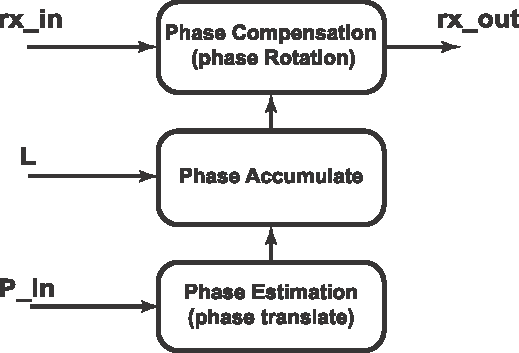
\includegraphics [width=0.4\columnwidth]{Figures/MSCR_RX_FFO.pdf}
\caption{Block diagram of frequency compensation module.}
\label{fig:FFO}
\end{figure}

\subsubsection{Fine STO Estimation}
\emph{FineSTO\_Est} estimates the starting sample of each OFDM symbol.
The RF front-end for MSCR need to access a wide range of frequencies, shown in Table~\ref{Tab:spec}. Depending on the standard being used, the CFO may be large, resulting in the presence of IFO.
Therefore, the implementation of \emph{FineSTO\_Est} is based on the algorithm presented in Chapter~\ref{chap:CFO} that is also robust to IFO.
The metric for fine STO estimation is expressed as:
\begin{equation}
\label{ProposedR}
S[d] =\sum_{m =0}^{L-1}   |r[d+m+L]|^2  |a[m]|^2,
\end{equation}
when $|a[m]|$ denotes the normalised amplitude of the preamble at the transmitter.

Fig.~\ref{fig:STO} shows the block diagram of fine STO estimation.
The metric is calculated based on a multiplierless correlation between received samples and transmitted preamble.
\emph{Peak Detect} finds the maximum value of correlation that is employed to accurately estimate the STO and \emph{Fine Time} determines the exact first sample of the next OFDM symbol (long preamble symbol).
However, multiplierless correlation is not flexible and the implementation depends on the preamble which is different for each standard.
Therefore, we employ PR module for the {FineSTO\_Est} module to obtain flexibility.
Each supported standard is implemented separately to a bitstream to be reconfigured at runtime by the \emph{CR engine} when the underlying standard is switched.
The PR region must be large enough to house the largest bitstream among the supported standards.
\begin{figure}
\centering
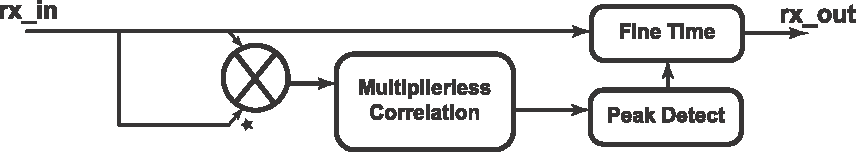
\includegraphics [width=0.6\columnwidth]{Figures/MSCR_RX_STO.pdf}
\caption{Block diagram of fine STO estimation module.}
\label{fig:STO}
\end{figure}

\subsubsection{Remove Cyclic Prefix}
\emph{RemoveCP} removes the cyclic prefix attached to each OFDM symbol.
The performance of this module depends on the length of CP $L_{CP}$ specified differently in each standards.
\emph{RemoveCP} consists of a counter to count from the beginning of each symbol and remove the CP samples if the counted value is smaller than $L_{CP}$
This module can be parameterised by adjusting $L_{CP}$ to support multiple standards.

\subsubsection{FFT}
\emph{FFT} is based on the Xilinx FFT/IFFT IP core, which supports modification of the FFT length at runtime to support different standards. When the standard is changed, the length of the FFT is modified using the relevant input. This reconfiguration completes within a few clock cycles.

\subsubsection{IFO Estimation and Channel Equalisation}
\emph{IFO\_Est\&Ch\_EstEqu} corrects IFO and performs channel equalisation.
IFO results in a cyclic shift in the frequency domain.
IFO is determined based on the method in Chapter~\ref{chap:CFO}:

\begin{equation}
\label{integerCFO}
\hat{\epsilon} =\underset{\tilde{\epsilon}}{\operatorname{argmax}}  \left|\sum_{k=0}^{N-1} Y^{*}[k-1] Y[k]  X^{*}[k-\tilde{\epsilon}]  X[k-1-\tilde{\epsilon}]\right|
\end{equation}
where $\epsilon$ denotes the value of IFO, $\hat{\epsilon}$, $\tilde{\epsilon}$ are estimated and trial values of $\epsilon$, respectively,
$Y(k)$ and $X(k)$ denote the $k^{th}$ frequency symbol index of the received subcarriers and the known transmitted preamble, respectively, and the OFDM symbol size $N$ is equal to the FFT size.

Fig.~\ref{fig:IFO} illustrates the block diagram of IFO estimation and channel equalisation.
\emph{IFO Correction} is performed effectively by cyclically shifting OFDM symbol corresponding to the estimated IFO estimation.

After compensating for IFO, the effects of the channel and residual STO must be taken into account to compensate the received sub-carriers.
Using information of the second preamble symbol, the effect of the channel can be estimated.
The estimation and compensation of channel and residual effects can be expressed as:
\begin{eqnarray}
\label{ChEqu}
Y[k] &=& X[k] * H[k] + N[k] \nonumber \\
H[k] &=& \frac{Y[k]-N[k]}{X[k]} \nonumber \\
\hat{H}[k] &=& \frac{Y[k]}{X[k]}\\
\label{ChCom}
\hat{R}[k] &=& \frac{R[k]}{\hat{H[k]}}
\end{eqnarray}
where $X[k]$, $Y[k]$ are the transmitted and received carriers in the preamble, respectively.
$H[n]$ represents for the channel and residual STO effect and $N[k]$ is the AWGN.
The equalization taps are estimated in (\ref{ChEqu}), and the compensation for received data carriers is given in (\ref{ChCom})
in which $R[k]$, $\hat{R}[k]$ denote received and compensated data carriers, respectively.

Since we use QPSK sub-carrier modulation, amplitude is not a concern. So, the complex division of channel estimation and compensation can be equivalently performed by multiplying by the conjugation of $X[k]$ and $\hat{H[k]}$, respectively.

This module depends on the second preamble that is specified differently for each standard.
Therefore, PR is used for the \emph{IFO\_Est\&Ch\_EstEqu} module to obtain effective standard-specific implementations.
\begin{figure}
\centering
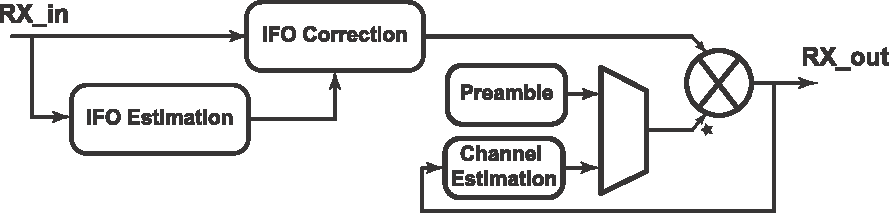
\includegraphics [width=0.7\columnwidth]{Figures/MSCR_RX_IFOCh.pdf}
\caption{The block diagram of IFO estimation and channel equalisation}
\label{fig:IFO}
\end{figure}

\subsubsection{Phase Tracking}
\emph{PhaseTrack} estimates the residual common phase error in each OFDM symbol after channel equalisation.
The \emph{PhaseTrack} implementation is based on an algorithm presented by Troya et al. \cite{Troya2007}.
The estimation is computed on the pilot symbols inserted in the OFDM symbol. The transmitted pilots are typically assigned
the values $\pm 1$. The residual phase error causes a phase rotation on received pilots.
\begin{eqnarray}
\label{PhaseTrack}
P_{k,l} = cos\theta_{l} -\alpha.k.sin \theta_{l} + j (sin\theta_{l} -\alpha.k.cos\theta_{l}),
\end{eqnarray}
where $P_{k,l}$ denotes the phase of received pilot which has frequency index $k$ in the $l^{th}$ OFDM symbol.
$cos\theta_{l} + j sin\theta_{l}$ is the residual common phase error of the $l^{th}$ OFDM symbol, and $\alpha$ is the slope of the phase distortion.
The residual common phase error is generally estimated for the supported standards as below:
\begin{eqnarray}
\label{CPE}
cos\theta_{l} &=& \frac{1}{N_P} \sum_{k \in S_P} \Re\{P_{k,l}\}, \\ \nonumber
sin\theta_{l} &=& \frac{1}{N_P} \sum_{k \in S_P} \Im\{P_{k,l}\}, \\ \nonumber
\end{eqnarray}
where $N_P$ denotes the number of received pilots employed for estimation, $S_P$ is a set of used pilot frequency indices.
The Fig.~\ref{fig:Phase} shows the block diagram of PhaseTrack. \emph{Pilot Extract} finds the employed pilots for phase tracking in the OFDM symbol based on allocation vector ($Alloc.~Bits$).
\emph{Phase Accumulator} computes the residual common phase error according to (\ref{CPE}).
The phase error is compensated for by multiplying the data carriers by the complex conjugate of the estimated common phase error.
To support multiple standards, $N_P$ is parameterised and $S_P$ can be determined through the allocation vector with the value shown in Table~\ref{tab:alloc_vec}

\begin{table}[h]
\centering
\caption{Allocation vector coding.}{
\label{tab:alloc_vec}
\renewcommand{\arraystretch}{1.3}
\begin{tabular}{@{}ll@{}}
\toprule
Subcarrier Type		&  Allocation Bits 	\\ \midrule
Null					&  00				\\
Data				&  10				\\
Positive pilot			&  01				\\
Negative pilot		&  11				\\
\end{tabular}
}
\end{table}
\begin{figure}
\centering
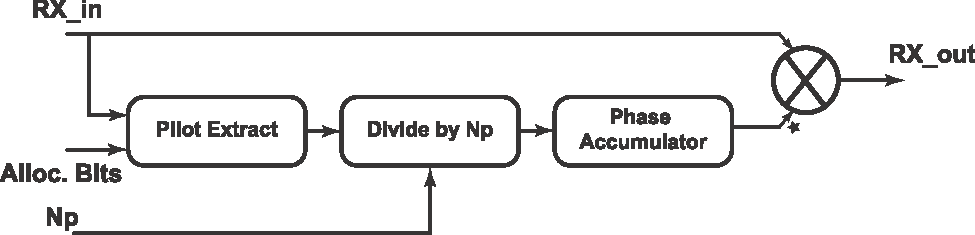
\includegraphics [width=0.7\columnwidth]{Figures/MSCR_RX_Phase.pdf}
\caption{Block diagram of phase tracking module.}
\label{fig:Phase}
\end{figure}

\subsubsection{Data symbol demodulation (\emph{DatSymDem})}
In the final step, the received bits are extracted from the data symbol by a data symbol demodulation block named \emph{DatSymDem}.
In the present implementation, this only supports QPSK modulation, but can be extended to support different data symbol modulations such as 16-QAM or 64-QAM in future, using the same basic interface.
All data symbols go through this module, and 2 bits are assigned to the output according to the sign bits of the real and imaginary parts of data symbol.


%---------------------------------------------------------------------------------
\section{Performance Analysis and Discussion}
\label{sec:PerAna}
%---------------------------------------------------------------------------------
\subsection{Latency and Stalling for PR-Based Baseband}

%\begin{figure*}[!t]
\begin{figure}
\centering{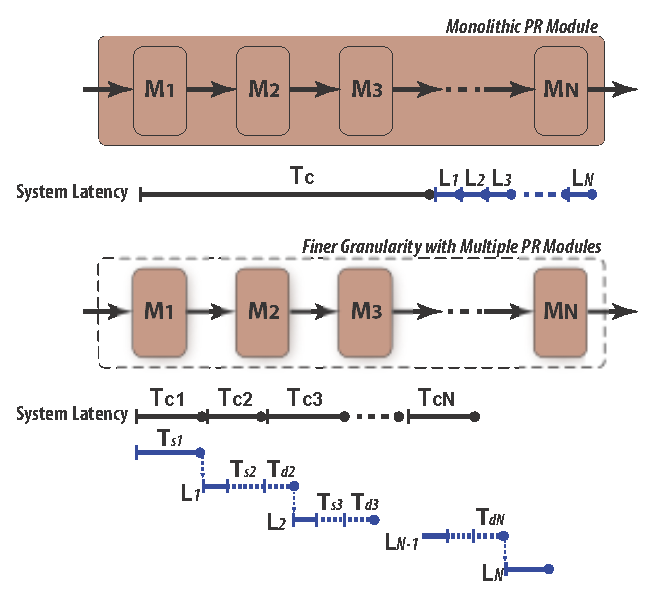
\includegraphics[width=0.8\columnwidth]{Figures/CRTiming.eps}}
\caption{Comparison of reconfiguration latency for a single and multiple PR modules.}
\label{fig:timing}
\end{figure}

One crucial challenge when implementing CR systems on reconfigurable hardware is long reconfiguration time when modifying the baseband.
PR can take a significant amount of time, especially for a large monolithic module.
In the case of the CR receiver, the system would have to stall during reconfiguration, potentially causing the loss of data packets and possibly even the loss of synchronisation.
A large FIFO would be required to store a stream of received samples long enough to overcome the reconfiguration latency when a large PR module is reconfigured.
A longer reconfiguration time would demand a larger FIFO, resulting in significantly increased hardware resource and power consumption.

We evaluate baseband latency for a monolithic PR module, as well as for a system employing a finer granularity with multiple PR modules, and a mix of PR and parameterised modules for the case when the system switches to a new baseband.
Fig.~\ref{fig:timing} illustrates this latency. We consider a system consisting of $N$ modules. $T_{c}$ refers to the reconfiguration time.
We assume that a module can not process data during its reconfiguration time.
$L_{i}$ is the computation latency of the $i^{th}$ module. Received data can, of course, be processed during the computation latency. In the case of a large monolithic PR module employed for the system, the system reconfiguration latency, $L_{sys}$, and halting time, $T_{hlt}$ that would require a FIFO to buffer received data which would otherwise be lost, is calculated as follow:

\begin{eqnarray}
\label{Mono}
L_{sys} &=& T_{c} + \sum_{i = 1}^{N}    (L_{i}) \nonumber \\
T_{hlt} &=& T_{c},
\end{eqnarray}

Finer granularity is possible by dividing the system into multiple sub-modules, each of which is implemented in a separate PR region. When a module is completely configured, it can process the received data while the following module is configured. Therefore, the system reconfiguration latency and halting time for the case of multiple PR modules can be calculated as follow;

\begin{eqnarray}
\label{Gran}
L_{sys} &=&  \sum_{i = 1}^{N} (T_{ci}) + T_{dN} + L_{N} \nonumber \\
T_{hlt} &=&  \sum_{i = 1}^{N}  (T_{si}),
\end{eqnarray}
where $T_{di}$ refers to the processing delay of the following module and $T_{si}$ is the stalling time to wait for configuration of the following module. If the computation latency of a module, $L_{i}$, is greater than the reconfiguration time of the following module,  $T_{ci+1}$, the following module has to delay operation by a duration $T_{di}$ before it receives input data for processing. Otherwise, the previous module is halted a duration $T_{si}$ until the following module is completely configured. The following module begins processing data just after its configuration is done ($T_{di} = 0$).

\begin{equation}
\label{DelayTime}
T_{di} = \begin{cases} Max(T_{ci}, T_{di-1}+L_{i-1}) - T_{ci}  	& i = 2..N, \\
						0 										& i = 1 \end{cases}  \\
\end{equation}
\begin{equation}
\label{HaltTime}
T_{si} = \begin{cases} T_{ci} - min(T_{ci}, T_{di-1}+L_{i-1}), 	&  i = 2..N, \\
					  T_{c1}									&  i=1 \end{cases}  \\
\end{equation}

Substituting the above equations into (\ref{Gran}),
\begin{eqnarray}
\label{Gran2}
L_{sys} &= & \sum_{i = 1}^{N}(T_{ci}) + L_{N} +   \nonumber \\
		& & (Max(T_{cN}, (Max( ... ) - T_{cN-1}) + L_{N-1}) - T_{cN})  \nonumber \\
T_{hlt} &= &\sum_{i = 1}^{N}(T_{ci})  -  \sum_{i = 2}^{N}  (min(T_{ci}, T_{di-1}+L_{i-1})),
\end{eqnarray}

We can see that system reconfiguration latency and halting time in the case of multiple PR modules is theoretically reduced thanks to being able to overlap the reconfiguration and data processing periods. Practically, the reconfiguration times are usually significantly greater than the processing latencies. This leads to $T_{di} = 0$ and  $min(T_{ci}, T_{di-1}+L_{i-1}) = L_{i-1}$ resulting in the approximated equations for (\ref{Gran2}) as below:
\begin{eqnarray}
\label{Gran3}
L_{sys} &= & \sum_{i = 1}^{N}(T_{ci}) + L_{N}    \nonumber \\
T_{hlt} &=  &\sum_{i = 1}^{N}(T_{ci})  -  \sum_{i = 1}^{N-1}  (L_{i}),
\end{eqnarray}

In addition, because of the optimisation in hardware compilation, the overhead of partitioning into multiple PR modules leads to the fact that $\sum_{i = 1}^{N}(T_{ci})$ is clearly greater than $T_{c}$, in (\ref{Mono}). Therefore, system reconfiguration latency, $L_{sys}$, and halting time, $T_{hlt}$ in (\ref{Gran2}) may be greater than that in (\ref{Mono}).
Generally, the finer granularity approach is only efficient in terms of system reconfiguration latency and halting time if the gain of overlapping the reconfiguration and data processing is greater than the overhead of partitioning into multiple PR modules.

Through the above analysis and comparison, we propose a new method employing a mix of PR modules and parameterised modules to obtain a significant reduction in system reconfiguration latency and halting time. For each module in the processing chain, commonalities across different operation modes are analysed. For modules requiring only minor modifications, parameterised versions are created.
For the $i^{th}$ module to be parameterised, the configuration time of this module can be eliminated because the parameterised modules can switch operating mode within one clock period. This approximately results in the following simplified equations;
\begin{eqnarray}
\label{Pro}
T_{ci} &\approx & 0   \nonumber \\
T_{si} &\approx & 0 \nonumber \\
T_{di} &\approx & T_{di-1} +  L_{i-1},
\end{eqnarray}

The above equations show the increasing efficiency of overlapping reconfiguration and data processing leading to a significant reduction in the system reconfiguration latency and halting time.

\subsection{Analysing the Proposed OFDM MSCR Approach}
We analyse the results of applying this method to the full receiver baseband  implemented on a xilinc Virtex~6 FPGA (XC6VLX240T).
We compare a large monolithic PR module, finer granularity PR, and the proposed mixture of PR and parameterisation.
\todo[inline]{Because slot based PR is widely used as well as being supported by Xilinx tools, we assume that slot-based PR is employed for performing PR.
All of the resources in the slot are consumed by the component, regardless of whether they are used in the computation or not. The configuration time for a component of a given slot is thus also constant, even if it small component.
There is some research~\cite{Sohanghpurwala2011} on reducing the wasted resources from unused logic in PR slots for small components that may reduce the reconfiguration time of such components. However, these approaches are just for limited FPGA devises, and require substantially more expert work to implement the designs.  
Furthermore, this improvement still does not help the overall reconfiguration latency because the overall latency has to take into account the worst case latency (i.e., the reconfiguration time of the largest components) when the system adapts from a standard to another.
}
To compute the configuration time of a PR module, we generate bitstreams for all modes.
The area of a PR region must satisfy the needs of the largest implementation it will house.
For the monolithic PR module, it is required that the PR module be able to contain the 802.22 OFDM baseband implementation, which is the largest receiver implementation among the three target implementations.

Similarly for the fine-grained approach, the configurations of the PR modules are computed based on the sub-modules of the 802.22 OFDM-based  implementation.
Table~\ref{tab:Resouces} reports the hardware resource usage for each sub-module and transmitter, receiver system for 802.22 on the Virtex~6 device. $M_1$, $M_2$, $M_3$, $M_4$, $M_5$, $M_6$, $M_7$, $M_8$ denote the functional modules of the OFDM based system: synchronisation, frequency compensation, fine STO estimation, remove CP, FFT, IFO estimation and channel equalisation, phase tracking, data symbol demodulation, respectively. $M_R$, $M_T$ are the monolithic receiver and transmitter sub-systems, respectively.
%Because we employ the multiplyless correlation for Fine STO estimation, DSP blocks are not used in this module but resulting in increased number of used slides.

We then determine the bitsteam size for each functional block according to the number of occupied CLB, DSP, BRAM columns that provide sufficient required resources for the block on FPGA floorplan. %\todo[inline]{How?}
Fig.~\ref{fig:Bitstream} illustrates the bitstream sizes of each PR module, which we use to calculate configuration time later. The bitstream sizes of the sub-modules are relatively small compared to the monolithic PR module for the receiver sub-system. The $M_3$ bitstream is the largest among the sub-modules. The bitstream of the receiver is nearly triple the size of the transmitter.
\begin{table}[hb]
	\centering
	\caption{Resources for 802.22 OFDM-based implementation}
	\label{tab:Resouces}
	\begin{tabular}{l|c|c|c}
        \hline \hline
    			  \makebox[4.2cm][c]{$modules$}	&  \makebox[2cm][c]{Slices}  &   \makebox[2cm][c]{DSP} &   \makebox[2cm][c]{BRAM} \\
	\hline
		$M_1$(\textit{Synch})     				& 498 		& 5	& 0 \\
		$M_2$(\textit{FreComp})				& 474		& 4 	& 0 \\
		$M_3$(\textit{FineSTO\_Est})			& 2414	& 0 	& 0 \\
		$M_4$(\textit{RemoveCP})			& 23  		& 0	& 0 \\
		$M_5$(\textit{FFT})	  			& 1179  	& 15	& 11 \\
		$M_6$(\textit{IFO\_Est\&Ch\_EstEqu})	  	& 1249 	& 6	& 0 \\
		$M_7$(\textit{Phasetrack})	  		& 523  	& 3	& 0 \\
		$M_8$(\textit{DatSymDem})	  		& 4	  	& 0	& 0 \\
		$M_R$(Receiver)  					& 6363  	& 33	& 11 \\
		$M_T$(Transmitter)					& 1668  	& 15	& 11 \\
	\hline \hline
    \end{tabular}
\end{table}

\begin{figure}
\centering
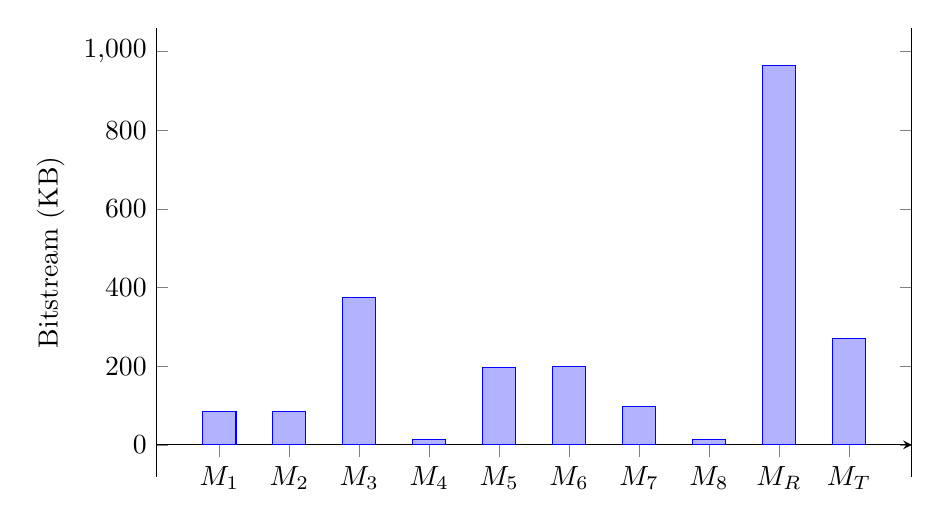
\begin{tikzpicture}[scale=1]
        \begin{axis}[
           axis x line=center,
           bar width=12pt,
           symbolic x coords={ $M_1$,$M_2$,$M_3$,$M_4$,$M_5$,$M_6$, $M_7$, $M_8$, $M_R$, $M_T$ },
           xtick=data,
	enlargelimits=true,
	ylabel={Bitstream (KB)},
	ylabel style={align=center},
%	xlabel={PR modules},
	ybar, x post scale=1.4]
            \addplot coordinates {
                ($M_1$,84.03) ($M_2$,84.03) ($M_3$,374.91) ($M_4$,14.54) ($M_5$,197.15) ($M_6$, 200.38)
                ($M_7$, 98.58) ($M_8$, 14.54) ($M_R$, 964.75) ($M_T$, 269.87)
               };
        \end{axis}
    \end{tikzpicture}
\caption{Bitstream sizes for PR modules.}
\label{fig:Bitstream}
\end{figure}

Processing latencies for functional modules are shown for the three standards in Fig.~\ref{fig:Latency}. We can see that 802.11 has the shortest latency because this standard uses the shortest FFT length, and hence the shortest symbol length for OFDM modulation.
It should be noted that during this latency the module still receives input data for processing.
The processing chain must be halted when the latency time has ended but the reconfiguration of the following module has not yet been completed.
The worst case halting time is a case of the shortest latency and the longest reconfiguration time.
Therefore, the latencies for 802.11 are used to calculate system halting time.
%The latency of the synchronisation module depends on the timing offset that is the duration from the time between receiving input samples and the time when the first sample of the coming frame is received. The synchronisation module does not output data if no frame is detected. Generally, the synchronisation latency is calculated as $L_{1} = \mathit{Offset} + \mathit{processing time}$ \todo[inline]{Don't you have a symbol for processing time defined earlier??}.
%To evaluate the processing latency of the synchronisation module, the timing offset is considered to be equal to 0. We will consider the presence of timing offset later for calculating the system halting time and FIFO requirements.
\begin{figure}
\centering
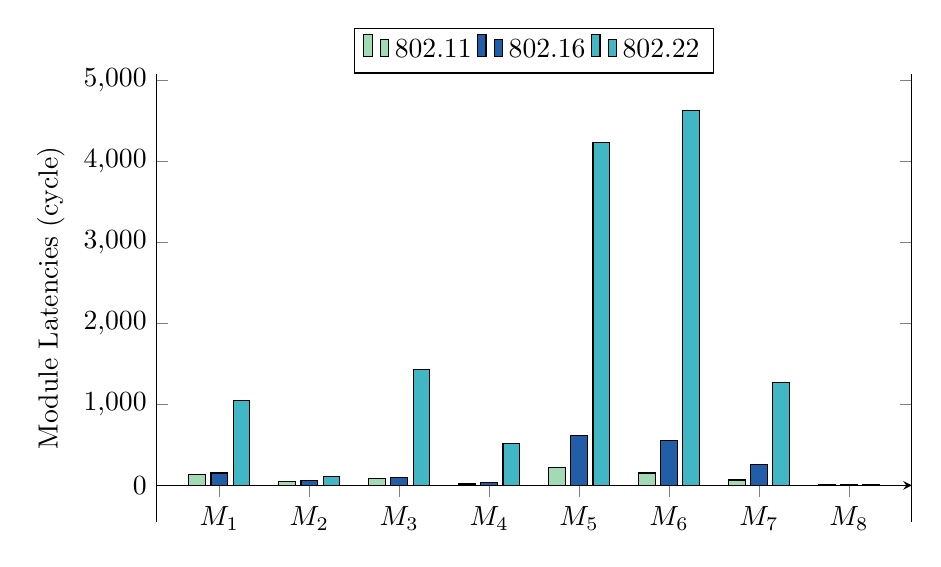
\begin{tikzpicture}
        \begin{axis}[
           ylabel={Module Latencies (cycle)},
	ylabel style={align=center},
           xtick = data,
	axis x line=center,
           bar width= 6pt,
%	nodes near coords,
	legend style={at={(0.5, 1)}, anchor=south, legend columns=-1},
           symbolic x coords={$M_1$,$M_2$,$M_3$,$M_4$,$M_5$,$M_6$, $M_7$, $M_8$ },
	enlargelimits=true,
  	ybar, x post scale=1.4]
	\addplot[fill=F1] coordinates {
		($M_1$,137) ($M_2$,45) ($M_3$,84) ($M_4$,17) ($M_5$,216) ($M_6$, 153) ($M_7$, 66) ($M_8$,11)
           };
	\addplot[fill=F2] coordinates {
		($M_1$,153) ($M_2$,61) ($M_3$,100) ($M_4$,33) ($M_5$,616) ($M_6$, 553) ($M_7$, 252) ($M_8$,11)
           };
 	\addplot[fill=F3] coordinates {
		($M_1$,1048) ($M_2$,110) ($M_3$,1428) ($M_4$,513) ($M_5$,4226) ($M_6$, 4617) ($M_7$, 1273) ($M_8$,11)
            };
   	\legend{802.11, 802.16, 802.22}
        \end{axis}
\end{tikzpicture}
\caption{The latency of sub-modules for three standards}
\label{fig:Latency}
\end{figure}

Partial reconfiguration is performed with a high throughput ICAP controller that supports a data rate of 380\,MBps, closet to the theoretical limit of the FPGA.
%We also factor in the required sampling frequency for each chosen standard.
We use a sampling frequency of 10 MHz (i.e. the clock period = 0.1 us) that is typically defined for the 802.11p standard. %\todo[inline]{These sentences contradict!}
Compute latency is calculated for the 802.11 standard, as shown in Fig.~\ref{fig:CfgLat}.
%The values of latency are scaled by a factor of 10 for better observation.
As can be seen, the latency is very small in comparison to the configuration time.%\todo[inline]{Does that mean the graph is wrong? if the scales are different, use different axes!}
It is clear that overlapping reconfiguration and data processing is not sufficient to hide reconfiguration delay, and so the finer granularity approach may not improve significantly over the monolithic PR module.
\begin{figure}
\centering
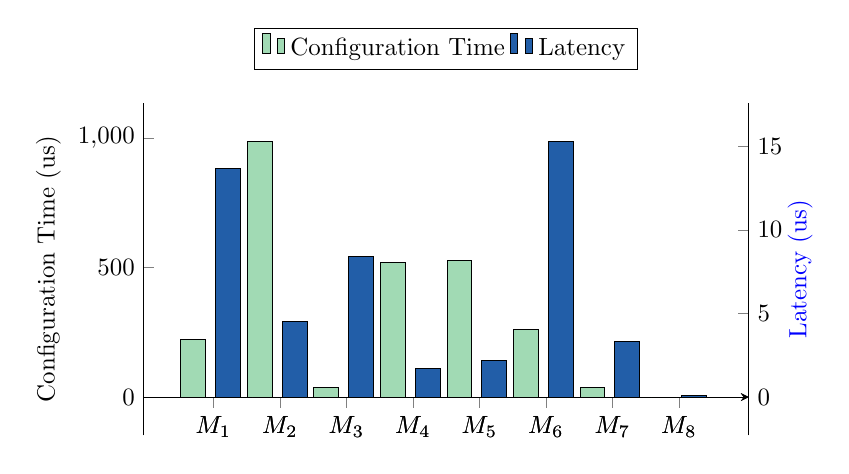
\begin{tikzpicture}[scale=0.9]
%        \begin{axis}[
%           ylabel={Time (us)},
%	ylabel style={align=center},
%           xtick = data,
%	axis x line=center,
%           bar width= 9pt,
%%	nodes near coords,
%	legend style={at={(0.5, 1)}, anchor=south, legend columns=-1},
%           symbolic x coords={$M_1$,$M_2$,$M_3$,$M_4$,$M_5$,$M_6$, $M_7$, $M_8$ },
%	enlargelimits=true,
%  	ybar, x post scale=1.4]
%	\addplot[fill=F1] coordinates {
%		($M_1$,221.14) ($M_2$,221.14) ($M_3$, 986.61) ($M_4$, 38.27) ($M_5$, 518.82) ($M_6$, 527.33) ($M_7$, 259.41) ($M_8$,38.27)
%           };
%	\addplot[fill=F2] coordinates {
%		($M_1$,137) ($M_2$,45) ($M_3$, 84) ($M_4$, 17) ($M_5$, 21.6) ($M_6$, 153) ($M_7$, 33) ($M_8$, 01)
%           };
%	\legend{Configuration Time, Latency}
%        \end{axis}
 	\begin{axis}[
           ylabel={Configuration Time (us)},
	ylabel style={align=center, color=black},
 	ymin=0,
	width= 0.6*\textwidth,
           xtick = data,
	axis x line=center,
           bar width=10pt,
           symbolic x coords={0, $M_1$,$M_2$,$M_3$,$M_4$,$M_5$,$M_6$, $M_7$, $M_8$ },
	enlargelimits=0.15,
    	axis y line*=none,
  	ybar, x post scale=1.5]
	\addplot[fill=F1,shift={(-8pt,0)}] coordinates {
 		($M_1$,221.14) ($M_2$,221.14) ($M_3$, 986.61) ($M_4$, 38.27) ($M_5$, 518.82) ($M_6$, 527.33) ($M_7$, 259.41) ($M_8$,38.27)
 		};
 	\end{axis}

	\begin{axis}[
           ylabel={Latency (us)},
	ylabel style={at={(1.05,0.5)}, color=blue},
 	ymin=0,
	width= 0.6*\textwidth,
           xtick = data,
	axis x line=center,
           bar width= 10pt,
	legend style={at={(0.5, 1.1)}, anchor=south, legend columns=2},
           symbolic x coords={0, $M_1$,$M_2$,$M_3$,$M_4$,$M_5$,$M_6$, $M_7$, $M_8$, 1},
	enlargelimits=0.15,
	axis y line*=right,
  	ybar, x post scale=1.5]
	\addplot [fill=F1] coordinates {($M_1$,0) ($M_2$,0) ($M_3$,0) ($M_4$, 0) ($M_5$, 0) ($M_6$, 0) ($M_7$, 0) ($M_8$, 0)};
	\addplot [fill=F2] coordinates {
 		($M_1$,13.7) ($M_2$,4.5) ($M_3$, 8.4) ($M_4$, 1.7) ($M_5$, 2.16) ($M_6$, 15.3) ($M_7$, 3.3) ($M_8$, 0.1)
		};
 	\legend{Configuration Time, Latency}
 	\end{axis}

\end{tikzpicture}
\caption{The configuration time and latency of sub-modules for OFDM-based MSCR system}
\label{fig:CfgLat}
\end{figure}

The system halting time is an accumulated value of the halting time in each module described in (\ref{HaltTime}). During the halting time, the processing chain is halted and a FIFO is required to buffer input samples. Because the halting time of the synchronisation module depends on the time when a new frame is detected. The timing offset must be taken into account. Given a scenario of a transmission, shown in Fig.~\ref{fig:tx-rx} when a standard switch is required, Both the transmitter and receiver spend time to reconfigure the system for the new baseband standard. In the proposed receiver, the synchronisation module is a parameterised module, so this module can change its function within a clock period and hence quickly process input samples. However, a new frame cannot be sent so quickly because the transmitter is still being reconfigured, resulting in a timing offset in the receiver. It is thus reasonable that the minimum timing offset can be chosen as the configuration time of the transmitter whose hardware characteristics were reported in Table~\ref{tab:Resouces}.
\begin{figure}
\centering
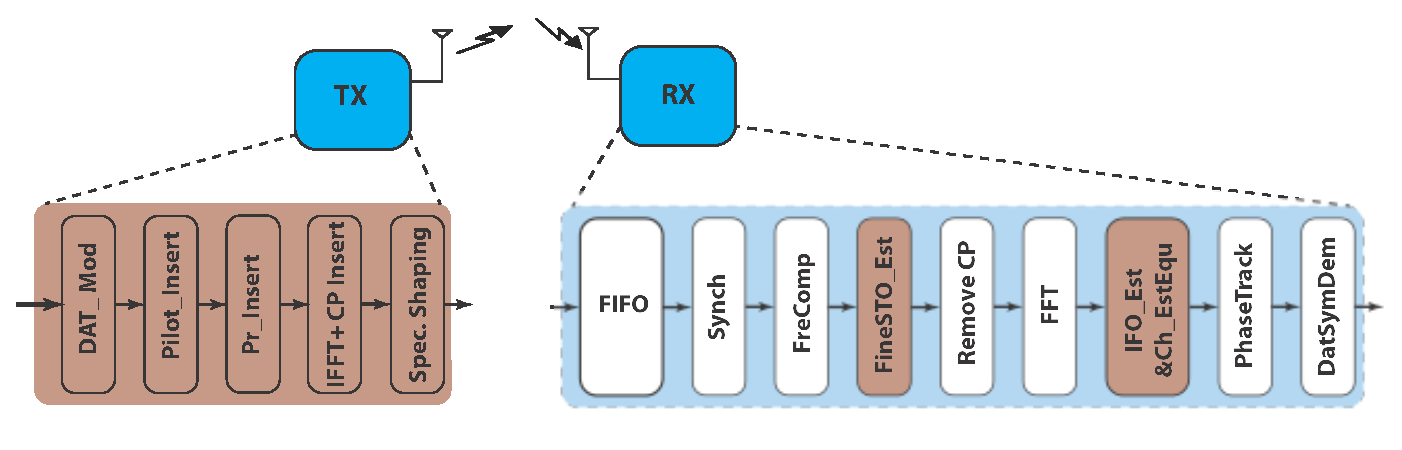
\includegraphics [width=1\columnwidth]{Figures/CR_Tx-Rx.eps}
\caption{A scenario of a transmission}
\label{fig:tx-rx}
\end{figure}

\definecolor{M1}{HTML}{FFFFd9}
\definecolor{M2}{HTML}{edF8b1}
\definecolor{M3}{HTML}{c7e9b4}
\definecolor{M4}{HTML}{7Fcdbb}
\definecolor{M5}{HTML}{41b6c4}
\definecolor{M6}{HTML}{1d91c0}
\definecolor{M7}{HTML}{225ea8}
\definecolor{M8}{HTML}{253494}
\definecolor{MR}{HTML}{081d58}
\begin{figure}
\centering
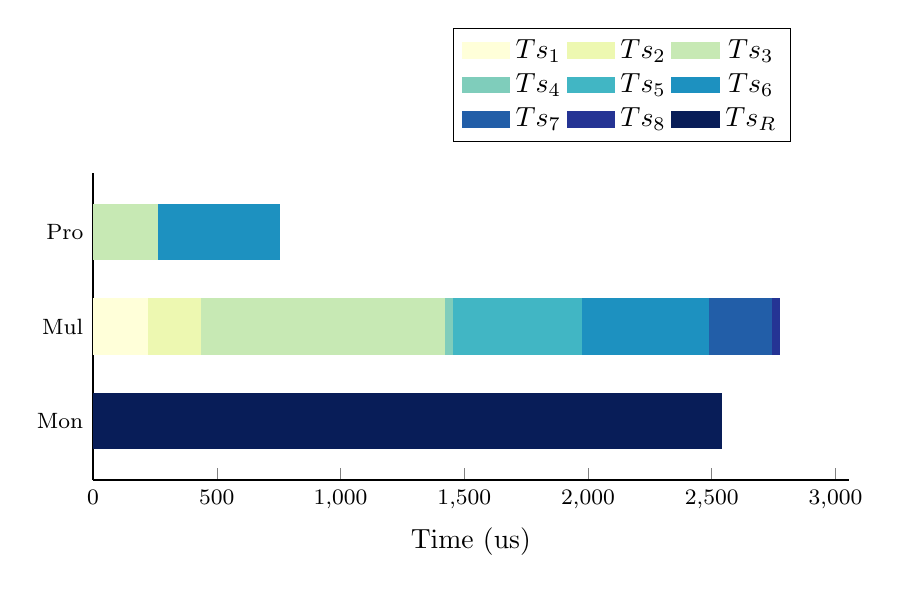
\begin{tikzpicture}
\begin{axis}[
	xbar stacked,
	legend style={at={(0.7, 1.1)}, anchor=south, legend columns=3},
    	ytick=data,
    	axis y line*=none,
    	axis x line*=bottom,
	tick label style={font=\footnotesize},
    	bar width= 20pt,
    	xlabel={Time (us)},
    	yticklabels={Mon, Mul , Pro},
    	xmin=0,
%    	xmax=600,
    	area legend,
    	y=12mm,
    	enlarge y limits={abs=0.625}, x post scale=1.4
	]
	\addplot [M1,fill=M1] coordinates {(0,0) (221.14,1) (0 ,2) };
	\addplot [M2,fill=M2] coordinates {(0,0) (214.28,1) (0,2) };
	\addplot [M3,fill=M3] coordinates {(0,0) (984.36,1) (258.22,2) };
	\addplot [M4,fill=M4] coordinates {(0,0) (034.07,1) (0,2) };
	\addplot [M5,fill=M5] coordinates {(0,0) (517.97,1) (0,2) };
	\addplot [M6,fill=M6] coordinates {(0,0) (516.53,1) (495.63,2) };
	\addplot [M7,fill=M7] coordinates {(0,0) (251.76,1) (0,2) };
	\addplot [M8,fill=M8] coordinates {(0,0) (034.97,1) (0,2) };
	\addplot [MR,fill=MR] coordinates {(2538.82,0) (0,1) (0,2)};
	\legend{$Ts_1$,$Ts_2$,$Ts_3$,$Ts_4$,$Ts_5$,$Ts_6$, $Ts_7$, $Ts_8$ , $Ts_R$}
\end{axis}
\end{tikzpicture}
\caption{ The halting time comparison of the system for three different approaches.}
\label{fig:Halt}
\end{figure}
%\todo[inline]{Fix the colours so they print ok in black and white.}

Fig.~\ref{fig:Halt} shows the system halting time of the three approaches. $Mon$, $Mul$, $Pro$ denote the halting time of the monolithic PR module approach, the multiple PR module approach, and the proposed approach, respectively. %\todo[inline]{Why not put them in the same order in the graph?}
$Ts_n$ is the halting time of the corresponding $M_n$ functional module. $Ts_R$ is the halting time of the monolithic receiver sub-system.

We can see that the halting time of the multiple PR module approach is greater than that of the monolithic PR module approach, because the gain achieved by overlapping reconfiguration and data processing is less than the overhead incurred by partitioning into multiple PR modules. The proposed approach can significantly reduce the halting time to less than one-third of that of the monolithic PR module approach. This results in a reduction in FIFO buffering requirements.
\begin{figure}
\centering
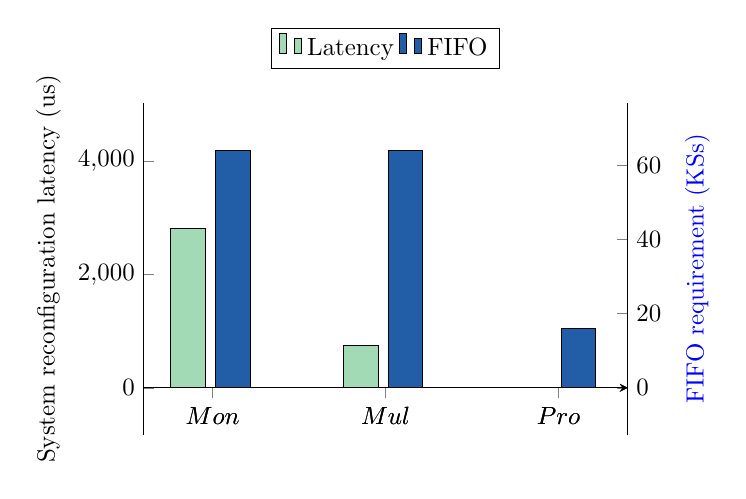
\begin{tikzpicture}[scale=0.9]
 	\begin{axis}[
           ylabel={System reconfiguration latency (us)},
	ylabel style={align=center, color=black},
 	ymin=0,
	width= 0.6*\textwidth,
           xtick = data,
	axis x line=center,
           bar width= 14pt,
           symbolic x coords={0, $Mon$, $Mul$, $Pro$},
	enlargelimits=0.2,
    	axis y line*=none,
  	ybar, x post scale=1.2]
	\addplot[fill=F1,shift={(-10pt,0)}] coordinates {($Mon$,4190.82) ($Mul$,2811.12) ($Pro$,753.97)  };
 	\end{axis}

	\begin{axis}[
           ylabel={FIFO requirement (KSs)},
	ylabel style={at={(1.1,0.5)}, color=blue},
 	ymin=0,
	width= 0.6*\textwidth,
           xtick = data,
	axis x line=center,
           bar width= 14pt,
	legend style={at={(0.5, 1.1)}, anchor=south, legend columns=2},
           symbolic x coords={0, $Mon$, $Mul$, $Pro$, 1},
	enlargelimits=0.2,
	axis y line*=right,
  	ybar, x post scale=1.2]
	\addplot [fill=F1] coordinates {($Mon$,0) ($Mul$,0) ($Pro$,0) };
	\addplot [fill=F2] coordinates {($Mon$,64) ($Mul$,64) ($Pro$,16)  };
 	\legend{Latency, FIFO}
 	\end{axis}

\end{tikzpicture}
\caption{A comparison of the three approaches in terms of system reconfiguration latency and FIFO requirements.}
\label{fig:LatFIFO}
\end{figure}

\begin{table}[hb]
	\centering
	\caption{Memory resources for 32 bit AXI4 interface FIFOs implementation}
	\label{tab:FIFOResouces}
	\begin{tabular}{c|c|c}
        \hline \hline
    			  FIFO size (KSs)&  18Kb BRAMs  & 36Kb BRAMs \\
	\hline
%		4     		& 0 	&  4 \\
		8			& 1	&  7 \\
		16			& 1	&  14  \\
		32			& 0 	&  29 \\
		64	  		& 0  & 58 \\
		128	  		& 0	 & 116 \\
	\hline \hline
    \end{tabular}
\end{table}
Fig.~\ref{fig:Halt} compares the three approaches in terms of system reconfiguration latency and FIFO buffering requirements. The system latencies are computed in the worst case which is the latency for the 802.22 standard. The FIFO requirements are calculated based on multiplying the sampling frequency by the halting time, followed by rounding up to the next power of two.  Table~\ref{tab:FIFOResouces} reports
required resources for 32 bit AXI4 interface FIFO implementation with some different availabe size configurations.
%\todo[inline]{Why do you have to round up? FIFOs can be any length}
The system reconfiguration latency of the proposed method is significantly reduced to 18~\% and 27~\% of the system reconfiguration latency of the monolithic PR module and the multiple PR module approaches, respectively. The FIFO requirement for the proposed approach is only 16 kilo-samples (KSs) while the other approaches require a FIFO to store up to 64~KSs.

\todo[inline]{A new subsection is added here for presenting system verification framework}
\section{System Verification}
\label{sec:SysVer}

This Section presents further evidence to demonstrate the correctness and performance of the Verilog HDL implementation. 
\begin{figure}
	\centering
	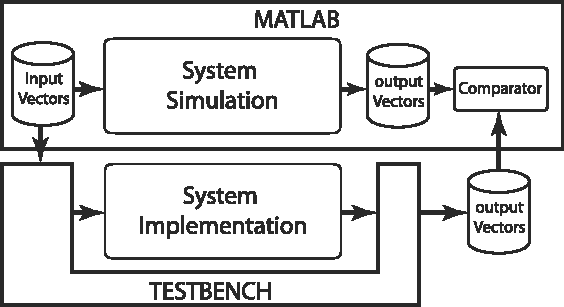
\includegraphics[width=0.9\columnwidth]{Figures/Veirification.pdf}
	\caption{The verification framework.}
	\label{fig:Ver}
\end{figure}
The overall framework, illustrated in Fig.~\ref{fig:Ver} is to work with parallel MATLAB and Verilog HDL implementations. The golden model simulation in MATLAB is used as the prototype with which the Verilog HDL code needs to comply, as well as providing a source for both random and non-random test vectors for each component of the FPGA code.
Common input vectors are used to perform OFDM modulation by both the system simulation and the system implementation. Test bench scripts have been written to send the input vectors from a database to the implemented system. Moreover, test bench scripts are also used to monitor the signals generated by the implementation and store them to a database as output vectors. These output vectors are then read by the MATLAB system for comparison against the corresponding vectors generated by the simulation.

\begin{figure}
	\centering
	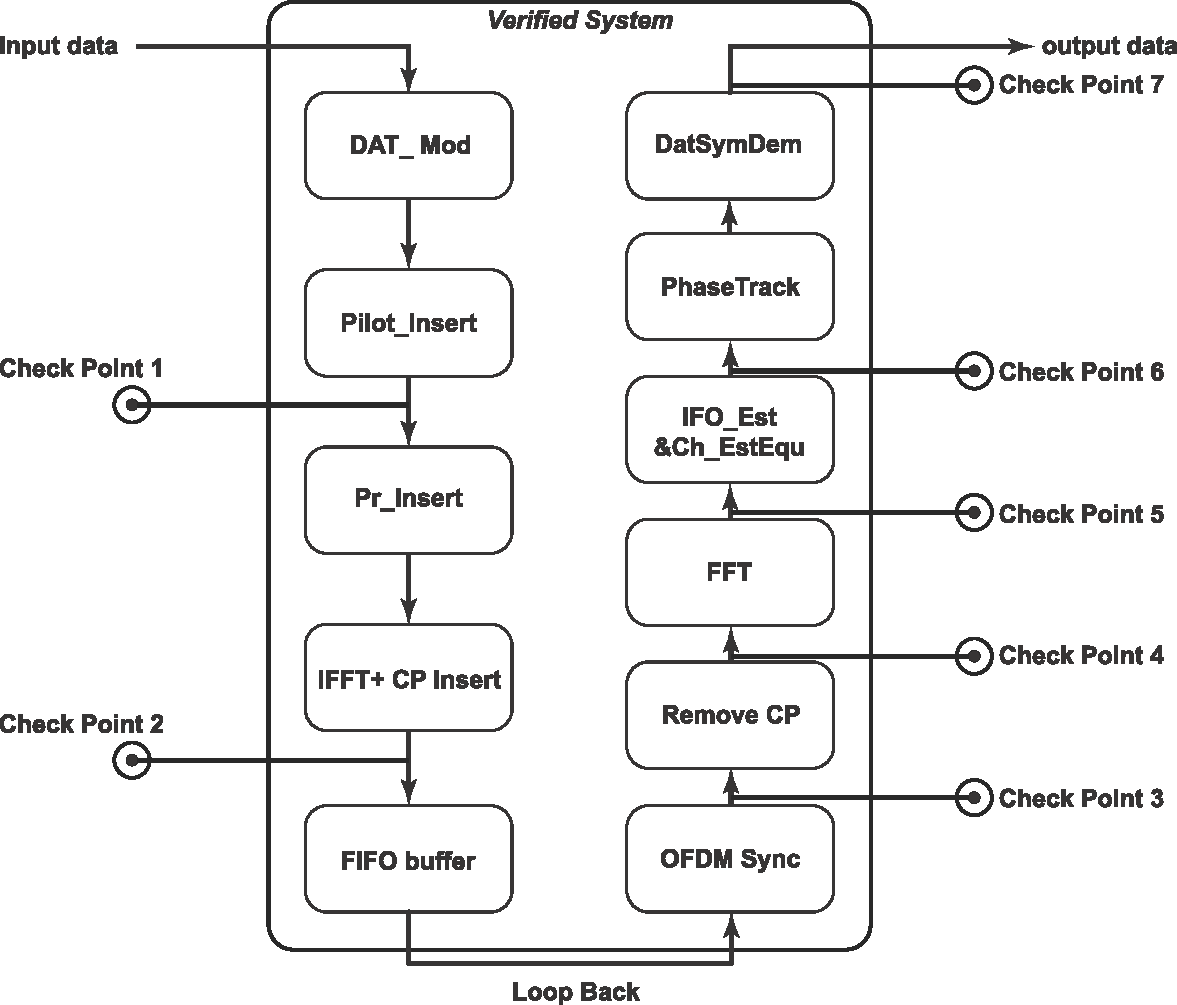
\includegraphics[width=0.9\columnwidth]{Figures/VerifiedSystem.pdf}
	\caption{The block diagram of verified system}
	\label{fig:VerSys}
\end{figure}

Fig.~\ref{fig:VerSys} shows a block diagram of the baseband system under verification. The necessary components are connected to a transmitter and a receiver. The output of the transmitter is buffered and connected to the receiver. It is immediately obvious that there are many intermediate check points located at the output of sub-modules that are observed within the implementation and compared to the simulation for verification.

The results of some of these verifications are shown in Fig.~\ref{fig:TX_Ver}, Fig.~\ref{fig:RX_Ver}, and Fig.~\ref{fig:Sys_Ver}.
These verify the system performing baseband modulation for one instance of an 802.11 signal. The nomenclature used is emph{MM\_sim} and \emph{MM\_rtl} which denote the output of the submodule named MM from the simulation and implementation respectively. Note from the waveforms plotted, the very close correspondence of the signal shapes illustrates the underlying correctness of the implementation.


\begin{figure}
	%\centering
	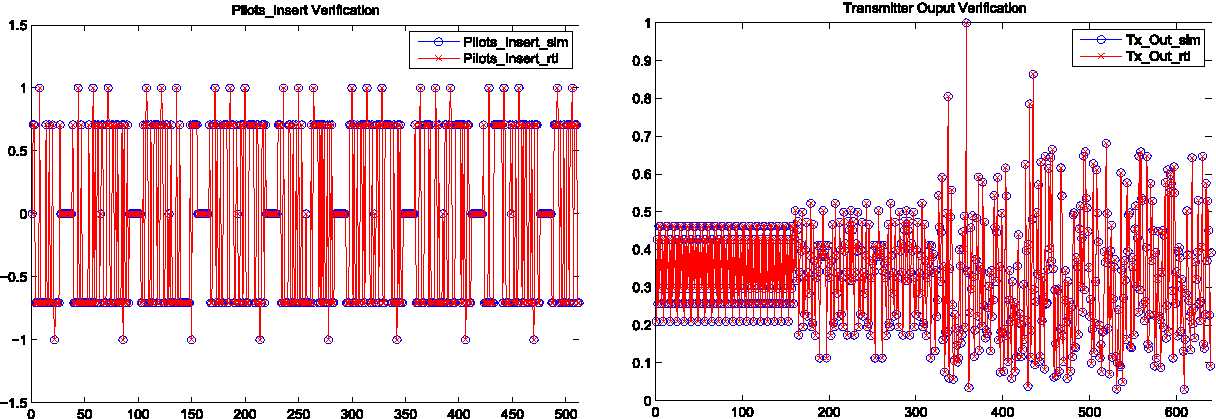
\includegraphics[width=1\columnwidth]{Figures/TX_Verification.pdf}
	\caption{The verification results of the transmitter.}
	\label{fig:TX_Ver}
\end{figure}

To consider more closely, Fig.~\ref{fig:TX_Ver} illustrates verification results from the transmitter. The left hand side figure compares the data symbols and the pilots being inserted into the OFDM symbols (i.e. the module input) while the right hand side shows a resulting OFDM signal (i.e. the module output). This includes the preamble as well as the OFDM symbols.

\begin{figure}
	%\centering
	\includegraphics[width=1\columnwidth]{Figures/Rx_Verification.pdf}
	\caption{The verification results of the receiver.}
	\label{fig:RX_Ver}
\end{figure}

Fig.~\ref{fig:RX_Ver} presents verification results from the receiver in a similar way. The top-left figure shows the synchronised signal, the top-right figure shows the signal with the cyclic prefix stripped. The bottom-left figure plots the demodulated data symbols after performing FFT. The output of the FFT contains a long preamble that is employed by the subsequent module which performs IFO estimation and channel equalisation. The output of this module is shown in bottom-right figure. Again all plots illustrate a close correspondence between simulation and implementation.

\begin{figure}
	%\centering
	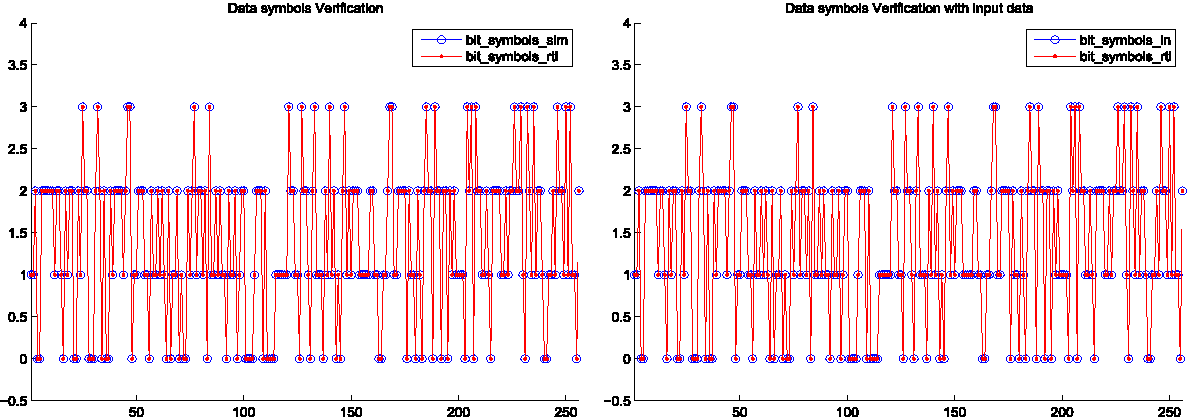
\includegraphics[width=1\columnwidth]{Figures/Sys_Verification.pdf}
	\caption{The verification results of the baseband system.}
	\label{fig:Sys_Ver}
\end{figure}

Fig.~\ref{fig:Sys_Ver} presents the observation of the bit streams at the system input and system output. The left hand figure shows the comparison of output bit streams from simulation and implementation. Because QPSK is used for data modulation, a data symbol is modulated with 2 data bits. Therefore, the value is presented from 0 to 3 corresponding to 00, 01, 10, 11 in binary. The right hand figure compares the input and output bit streams. The data bit stream is modulated at OFDM based band and then demodulated. The input and output streams are identical to each other.
 
Through this careful verification framework, and making use of extensive test benches  the performance of the system implementation is verified with regard to the golden reference model in MATLAB.  

%---------------------------------------------------------------------------------
\section{Summary}
%---------------------------------------------------------------------------------
We have shown that configuring a radio baseband composed of multiple modules can be made more efficient in terms of time, and buffering requirements, by mixing parameterisation and PR.
Implement the whole baseband as a single PR module leads to long reconfiguration time, during which no processing can be performed, and hence significant FIFO buffering to prevent loss of samples in the receiver.
Breaking the baseband chain into multiple PR modules could be beneficial as it would allow individual modules to start processing as they complete their reconfiguration, overlapping this processing with the reconfiguration of the next module. However, since reconfiguration time is significantly higher than the computational latency, we find that the benefit is outweighed by the overhead of multiple PR modules.
Our proposed approach only applies PR to modules where different modes are very different in hardware, with other modules designed to be parameterisable. As a result, overall halting time is reduced by more than half.
The FIFO buffering requirement of the proposed method is also decreased to 25~\% of that required for the other methods.
We are working on finalising a demonstrator for this approach.